% =====================================================================
%  §6.4–6.6  （原文 p41–p48 开头）
%  接 ch06（§6 的 \section 与 6.1–6.3）
% =====================================================================
\subsection{子复形上的 \texorpdfstring{$\Ainf$}{A∞}-结构}

本节中，我们要把 \cite{GS} 与 \cite{Me} 的若干结果改写成一种便于使用的形式。

设 $(A,m_n)$，$n\ge1$，是一个非幺 $\Ainf$-代数，$\Pi:A\to A$ 是一个与微分 $d=m_1$ 交换的幂等映射。
换言之，$\Pi$ 是零次线性映射，满足 $d\Pi=\Pi d$、$\Pi^2=\Pi$。假设还给定了一个同伦
$H:A\to A[-1]$，使得 $1-\Pi=dH+Hd$。记 $\Pi$ 的像为 $B$。于是我们有嵌入 $i:B\to A$ 与投影
$p:A\to B$，满足 $\Pi=i\circ p$。

我们按下述方式引入一列线性运算 $m_n^B:B^{\otimes n}\to B[2-n]$\footnote{在某个特殊情形下，类似的
公式已出现在 \cite{Go} 中。}：
\begin{enumerate}[label=\alph*),leftmargin=2.6em]
  \item $m_1^B:=d^B=p\circ m_1\circ i$；
  \item $m_2^B=p\circ m_2\circ(i\otimes i)$；
  \item $m_n^B=\sum_T\pm m_{n,T}$，$n\ge3$。
\end{enumerate}
这里的求和取遍所有定向平面树（oriented planar tree）$T$，它们有 $n+1$ 个尾顶点（包括根顶点），
并且 $T$ 的每个内顶点的（定向）度数 $|v|$（即入边的条数）至少为 $2$。为了描述线性映射
$m_{n,T}:B^{\otimes n}\to B[2-n]$，我们需要作一些准备。考虑另一棵树 $\bar T$，它由 $T$ 在每条
内边上插入一个新顶点得到。于是 $\bar T$ 的内顶点分为两类：「旧」顶点，与 $T$ 的内顶点重合；
以及「新」顶点，在几何上可以看成 $T$ 的内边的中点。

给 $\bar T$ 的每个尾顶点配上嵌入 $i$；给每个「旧」顶点 $v$ 配上 $m_k$，其中 $k=|v|$；给每个
「新」顶点配上同伦算子（homotopy operator）$H$；给根配上投影算子（projector）$p$。然后沿树向根的
方向走，把各顶点所配的映射复合起来，就得到映射 $m_{n,T}$。$T$ 与 $\bar T$ 的一个例子如下：

\begin{center}
  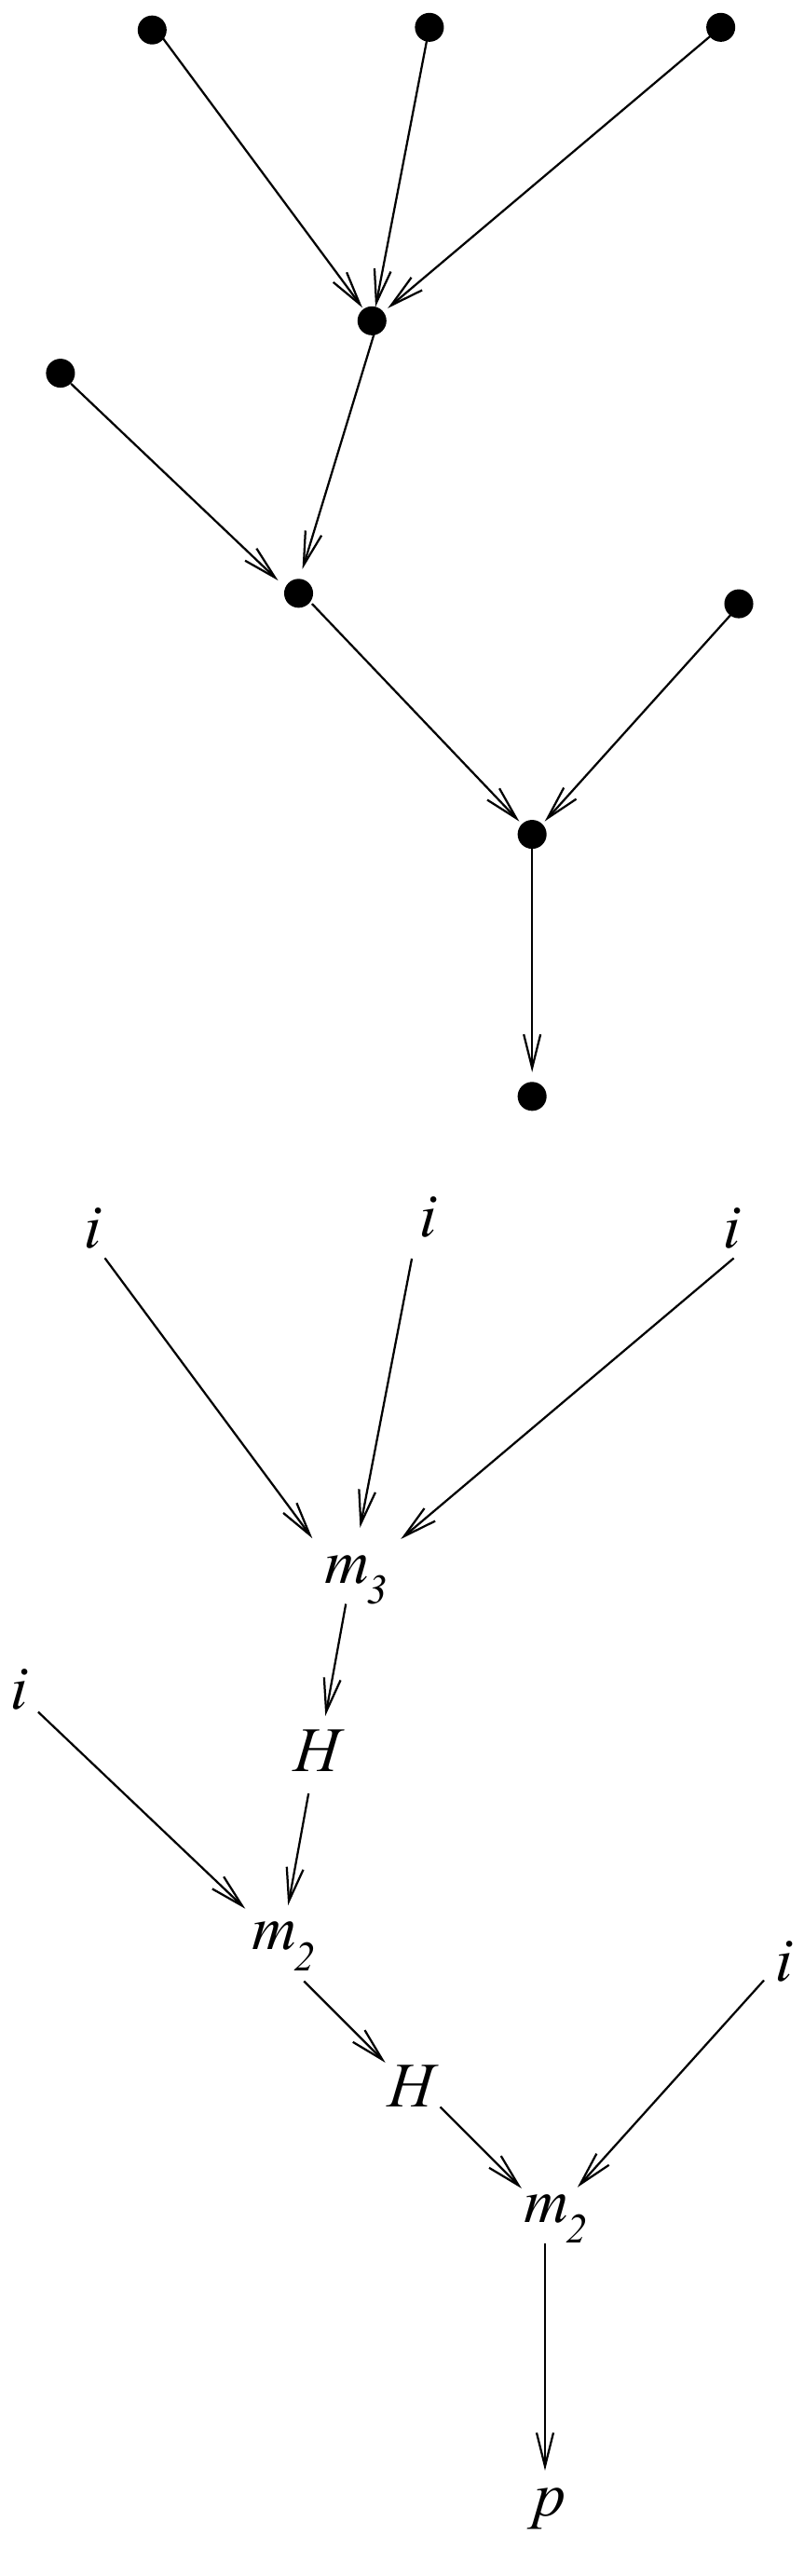
\includegraphics[width=3.65 cm]{figures/fig7_p42_trees_T_Tbar}
\end{center}

\begin{prp}
线性映射 $m_1^B$ 定义了 $B$ 中的一个微分。
\end{prp}

\begin{proof}
显然。
\end{proof}

\begin{thm}
序列 $m_n^B$，$n\ge1$，给出 $B$ 上的一个 $\Ainf$-代数结构。
\end{thm}

\begin{proof}[证明概要]
证明相当直接，因此我们只简要说明计算的主要步骤。

首先注意到，$p$ 与 $i$ 都是复形的同态。为证明定理，对给定的 $n\ge2$，我们把每个被加项
$m_{n,T}$ 换成一个不同的项，然后用两种不同的方式计算所得的结果。考虑一族树
$\{\bar T_e\}_{e\in E(\bar T)}$，其中 $\bar T_e$ 由 $\bar T$ 如下得到：
\begin{enumerate}[label=\alph*),leftmargin=2.6em]
  \item 把边 $e$ 从内部劈成两条边，即在 $e$ 内插入一个新顶点 $w_e$；
  \item $\bar T$ 的其余部分保持不变。
\end{enumerate}
我们把 $d=m_1$ 配给顶点 $w_e$，其余配置一概不动。这样就得到一个映射
$m_{n,\bar T_e}:B^{\otimes n}\to B[3-n]$。

考虑如下之和（带适当的符号）：
\[
  \hat m_n^B=\sum_T\sum_{e\in E(\bar T)}\pm m_{n,\bar T_e}.
\]
我们可以用两种方式计算它：一是利用关系式 $1-\Pi=dH+Hd$，二是利用 $A$ 的 $\Ainf$-结构所给出的
$d(m_j)$ 的公式，$j\ge2$。对关系式 $1-\Pi=dH+Hd=:d(H)$ 的情形，得到
\[
  \hat m_n^B=d(m_n^B)-m_n^{B,\Pi}+m_n^{B,1},
\]
其中 $m_n^{B,\Pi}$ 的定义与 $m_n^B$ 类似，唯一的差别是：对某条边 $e\in E_i(T)$，我们在相应的新顶点上
配以算子 $\Pi$ 而不是 $H$。类似地，若在新顶点上配以 $1=\id_A$ 而不是 $H$，就得到被加项
$m_n^{B,1}$ 的定义。而 $d(m_j)$ 的公式是 $m_l$（$l<j$）的二次表达式。这给出另一个恒等式
\[
  \hat m_n^B=m_n^{B,1}.
\]
于是 $d(m_n^B)=m_n^{B,\Pi}$，而这恰好就是族 $(m_n^B)_{n\ge1}$ 的 $\Ainf$-约束。
\end{proof}

此外，用类似的技术可以证明下述结果。

\begin{prp}
存在典范的 $\Ainf$-态射 $g:B\to A$，它给出 $\Ainf$-代数的拟同构。
\end{prp}

为读者方便起见，我们给出 $g$ 的一个典范取法的显式公式。算子 $g_1:B\to A$ 取为嵌入 $i$。对
$n\ge2$，定义 $g_n$ 为各项 $g_{n,T}$ 之和，求和取遍所有具有 $n+1$ 个尾的平面树 $T$。每一项
$g_{n,T}$ 与上面定义的 $m_{n,T}$ 类似，唯一的差别是：我们在根顶点上配以算子 $H$ 而不是 $p$。

也可以显式地构造 $\Ainf$-拟同构 $A\to B$。

\begin{yizhu}[同调扰动理论]
\cite{GS} 指 Gugenheim--Stasheff，\cite{Me} 指 Merkulov。把 $\Ainf$-结构沿一对「投影与同伦」
$(\Pi,H)$ 从 $A$ 转移到子复形 $B$ 上的这套手续，就是所谓同调扰动理论（homological perturbation
theory）。其要点在于：$B$ 上 $\Ainf$-约束中不闭合的部分，恰好被同伦等式 $1-\Pi=dH+Hd$ 吸收；
定理 3 的证明就是把这一吸收逐项写出来。
\end{yizhu}

\begin{rmk}
a) 类似的构造对任意非幺 $\Ainf$-范畴都适用。此时需要对每个分次态射空间 $\Hom(X,Y)$ 给定投影算子
$\Pi_{X,Y}$ 与同伦 $H_{X,Y}$。所有公式都与 $\Ainf$-代数的情形相同。所得的 $\Ainf$-范畴，其态射空间
由 $\Pi_{X,Y}(\Hom(X,Y))$ 给出，与原范畴等价。我们以后会用到这一事实。

b) 命题 4 与命题 5 应当在 operad 上的代数这一远为一般的情形下也成立（例如见 \cite{M}）。
\end{rmk}

\subsection{Morse 理论中的投影算子与同伦}

我们想把子复形上 $\Ainf$-结构的公式应用于定理 2 的证明。为此需要把 Morse 复形等同于 de Rham
复形的一个直和项。我们的进路基于 Harvey 与 Lawson 的想法（见 \cite{HL}）。

设 $Y$ 是紧的定向光滑流形，$\dim Y=n$。我们把流（current）空间 $D'(Y)$ 与分布值微分形式的空间
等同起来。连续线性算子 $\Omega^*(Y)\to D'(Y)$ 由它们的 Schwartz 核给出，而核是 $D'(Y\times Y)$ 的
元素。磨光算子 $D'(Y)\to\Omega^*(Y)$ 的核落在 $\Omega^*(Y\times Y)\subset D'(Y\times Y)$ 中。

对任意有限体积的定向子流形 $Z\subset Y$，$\dim Z=k$，我们联系一个典范的 $n-k$ 次流 $[Z]$
（也就是说，可以把光滑 $k$-形式在 $Z$ 上积分）。

设 $g_Y$ 是 $Y$ 上的黎曼度量，$f$ 是 Morse--Smale 函数。梯度流 $\exp(t\grad(f))$，$t\ge0$，给出
作用在 $\Omega^*(Y)$ 上的单参数半群：$\psi^t(\alpha)=\exp(t\grad(f))^*(\alpha)$。$\psi^t$ 的
Schwartz 核是 $[G_t]$，其中流形 $G_t\subset Y\times Y$ 由
$G_t:=\operatorname{graph}(\exp(t\grad(f)))$ 给出。我们还有恒等式
\[
  \id-\psi^t=dH^t+H^td,
\]
其中 $H^t:\Omega^*(Y)\to\Omega^*(Y)\subset D'(Y)$ 是由分布核 $[Z_t]$ 定义的 $-1$ 次线性算子，
$Z_t:=\cup_{0\le t'\le t}\operatorname{graph}(\exp(t'\grad(f)))$。

\cite{HL} 中验证了：当 $t\to+\infty$ 时这一图景有极限。也就是说，流 $[G_t]$ 与 $[Z_t]$ 的极限存在：
\begin{align*}
  [G_\infty]&=\lim_{t\to+\infty}[G_t]=\sum_{x\in\operatorname{Cr}(f)}[S_x]\times[U_x],\\
  [Z_\infty]&=\lim_{t\to+\infty}[Z_t]=\bigl[\cup_{0\le t<+\infty}G_t\bigr].
\end{align*}

对应于这些核的线性算子 $\psi^\infty$（零次）与 $H^\infty$（$-1$ 次）把 $\Omega^*(Y)$ 映入
$D'(Y)$，并满足恒等式
\[
  i-\psi^\infty=dH^\infty+H^\infty d,
\]
其中 $i:\Omega^*(Y)\to D'(Y)$ 是自然嵌入。由 de Rham 定理，这个嵌入是复形的拟同构，因此
$\psi^\infty$ 也是。从道德上说，$\Pi_\infty:=\psi^\infty$ 应当被看成一个投影算子。像
$\Pi_\infty(\Omega^*(Y))\subset D'(Y)$ 与 $\oplus_{x\in\operatorname{Cr}(f)}\R\cdot[U_x]$ 重合。我们有
\[
  \Pi_\infty(\alpha)=\sum_{x\in\operatorname{Cr}(f)}\Bigl(\int_{S_x}\alpha\Bigr)\cdot[U_x]
  =\sum_{x\in\operatorname{Cr}(f)}\int_Y(\alpha\wedge[S_x])\cdot[U_x].
\]

此外，算子 $\Pi_\infty$ 与微分交换。因此复形 $\Pi_\infty(\Omega^*(Y))$ 是 $D'(Y)$ 的有限维子复形，
同构于 Morse 复形 $M^*(Y,f)$。事实上它与 $\Omega^*(Y)$ 及 $D'(Y)$ 都拟同构。Harvey 与 Lawson
就是这样证明 de Rham 上同调同构于 Morse 复形的上同调的。

为了构造真正的投影算子与同伦，我们如下进行。设 $\rho_\delta$，$\delta\to0$，是 $Y\times Y$ 上一族
光滑闭 $n$-形式，使得 $\Supp(\rho_\delta)$ 落在对角线 $\operatorname{diag}\subset Y\times Y$ 的开
$\delta$-邻域 $N_\delta$ 内，且 $\rho_\delta$ 在 $H^n_c(N_\delta,\R)$ 中的上同调类与
$[\operatorname{diag}]$ 的相同。

我们定义 $R_\delta:D'(Y)\to\Omega^*(Y)$ 为由核 $\rho_\delta$ 给出的积分算子。

\begin{lmm}
\begin{enumerate}[label=\arabic*),leftmargin=2.6em]
  \item 算子 $R_\delta$ 是复形的同态。
  \item 若 $Z_1,Z_2\subset Y$ 是两个有限体积的定向子流形，它们横截相交于有限多个点，
  $\dim Z_1+\dim Z_2=\dim Y$，且 $\overline{Z_1}\cap\overline{Z_2}=Z_1\cap Z_2$，则对充分小的
  $\delta$ 有
  \[
    \int_Y R_\delta([Z_1])\wedge R_\delta([Z_2])=\deg(Z_1\cap Z_2)\in\Z.
  \]
  \item 存在线性算子 $h_\delta:\Omega^*(Y)\to\Omega^*(Y)$，其核的支集含于 $N_\delta$，波前集
  $WF(h_\delta)$ 是对角线 $\operatorname{diag}\subset Y\times Y$ 的余法丛，并且
  \[
    dh_\delta+h_\delta d=\id-(R_\delta)|_{\Omega^*(Y)}.
  \]
\end{enumerate}
\end{lmm}

\begin{proof}
第 1) 部分由 $\rho_\delta$ 是闭流这一事实推出。第 2) 部分由 $R_\delta$ 只把 $Z_i$（$i=1,2$）的支集
改变 $O(\delta)$ 这一事实推出。为证第 3) 部分，注意算子 $\id$ 与 $(R_\delta)|_{\Omega^*(Y)}$ 都保持
光滑形式空间 $\Omega^*(Y)$，且 $\rho_\delta$ 与 $[\operatorname{diag}]$ 同调。
\end{proof}

\begin{yizhu}[流与 Schwartz 核]
这里按 \cite{HL} 的做法，把微分形式嵌入流空间 $D'(Y)$，线性算子则用它在 $Y\times Y$ 上的 Schwartz
核（一个流或形式）来表示：核的支集越靠近对角线，算子越光滑。第 3) 条中的波前集条件保证了两个核可以
作纤维乘积 $\boxtimes$，这正是紧接着的同伦算子 $H_\delta$ 得以良定义的原因。
\end{yizhu}

设 $x,y\in\operatorname{Cr}(f)$ 是两个具有相同 Morse 指标的临界点。则 $\deg(S_x\cap U_y)=\delta_{xy}$
（Kronecker 符号）。由引理第 2) 部分，对充分小的 $\delta$ 得到恒等式
\[
  \int_Y R_\delta([S_x])\wedge R_\delta([U_y])=\delta_{xy}.
\]
这蕴含下述结果。

\begin{prp}
对充分小的 $\delta$，用公式
\[
  \Pi_\delta(\alpha)=\sum_{x\in\operatorname{Cr}(f)}\Bigl(\int_Y\alpha\wedge R_\delta([S_x])\Bigr)
  \cdot R_\delta([U_x])
\]
定义线性算子 $D'(Y)\to\Omega^*(Y)$。则
\begin{enumerate}[label=\arabic*),leftmargin=2.6em]
  \item 若 $\alpha\in\Omega^*(Y)$，则 $\Pi_\delta^2(\alpha)=\Pi_\delta(\alpha)$，且
  $\Pi_\delta d=d\Pi_\delta$。
  \item 像 $\Pi_\delta(M^*(Y,f))$ 是 $\Omega^*(Y)$ 中的子复形，典范同构于 Morse 复形
  $M^*(Y,f)$。
\end{enumerate}
\end{prp}

我们把同伦算子 $H_\delta:\Omega^*(Y)\to\Omega^*(Y)[-1]$ 定义为由核
\[
  (R_\delta\boxtimes R_\delta)[Z_\infty]+(h_\delta\boxtimes h_\delta)([\operatorname{diag}])
\]
给出的积分算子。（最后一项之所以有意义，是因为对 $h_\delta$ 的波前集作了上述条件。）容易验证下述
恒等式成立：
\[
  \id-\Pi_\delta=dH_\delta+H_\delta d.
\]
于是我们得到一族由 $\delta$ 参数化的同伦与投影算子。

\begin{rmk}
可以用另一个典范元素 $\sum_{x\in\operatorname{Cr}(f)}[S_x]\otimes R_\delta([U_x])$ 来定义投影算子
$\Pi_\delta$，而不必像我们这样用
$\sum_{x\in\operatorname{Cr}(f)}R_\delta([S_x])\otimes R_\delta([U_x])$。上述命题对新的典范元素同样成立。
\end{rmk}

前一个构造有一个变体，它在下一小节中会用到。也就是说，我们从一个微分 $n+1$-形式 $\rho$ 出发，
它定义在 $Y\times Y\times(0,1)$ 上，使得 $\Supp(\rho)$ 对所有充分小的 $\delta\in(0,1)$ 都含于
$\sqcup_{\delta>0}(N_\delta,\delta)$ 中，并且 $\rho$ 在 $H^n_c(Y\times Y\times(0,1))$ 中定义了与
$[\operatorname{diag}]\times(0,1)$ 相同的上同调类。

现在考虑空间 $\Omega^*_0(Y):=\varinjlim_{\delta\to0}\Omega^*(Y\times(0,\delta))$ 与
$D'_0(Y):=\varinjlim_{\delta\to0}\Omega^*(0,\delta)\hat\otimes D'(Y)$。容易看出，两个复形
$\Omega^*_0(Y)$ 与 $D'_0(Y)$ 都拟同构于 $\Omega^*(Y)$。

\begin{yizhu}[一处上标次数]
原文写 $H^n_c(Y\times Y\times(0,1))$。但 $\rho$ 是 $n+1$-形式，闭形式的上同调类应落在
$H^{n+1}$ 中；若把 $[\operatorname{diag}]\times(0,1)$ 理解为流之积
$[\operatorname{diag}]\wedge[0,1]$（次数 $n+1$），则此处指标应为 $n+1$。译文照录原文，存疑待考。
\end{yizhu}

\subsection{\S6.3 中定理的证明}

为简单起见，我们假定所有局部系都是平凡的且秩为一。一般情形完全类似。

我们将构造连接 $DR(Y)$ 与 $M(Y)$ 的如下 $\Ainf$-等价链：
\[
  DR(Y)\hookrightarrow DR_0(Y)\hookleftarrow DR_0^{tr}(Y)\hookleftarrow DR_0^{tr,\Pi}(Y)
  \hookleftarrow M(Y).
\]
所有这些范畴的对象类都相同，且所有函子在对象上都是恒等的。

$\Ainf$-预范畴 $DR_0(Y)$ 实际上是一个 dg-范畴，即所有对象序列都横截，当 $k\ge3$ 时复合 $m_k$
为零，并且它有严格单位态射。空间 $\Hom_{DR_0(Y)}(f_0,f_1)$ 定义为
$\varinjlim_{\delta\to0}\Omega^*(Y\times(0,\delta))=\Omega^*_0(Y)$。显然，态射空间不依赖于对象。
利用微分形式的外积，我们把 $DR_0(Y)$ 变成 $\C$ 上的 dg-范畴。存在自然的函子
$DR(Y)\to DR_0(Y)$，它在对象上是恒等映射；在态射上，它是 $\Omega^*(Y)$ 作为 $Y\times(0,\delta)$
上形式之子空间的自然嵌入，而这些形式是 $Y$ 上形式的拉回。显然它给出 $\Ainf$-范畴的等价。

$\Ainf$-预范畴 $DR_0^{tr}(Y)$ 定义为 $DR_0(Y)$ 的满子范畴，它与后者的差别仅在于横截序列的选取。
也就是说，我们在 $DR_0^{tr}(Y)$ 中使用与 Morse 范畴相同的横截性概念。

下一个 $\Ainf$-预范畴 $DR_0^{tr,\Pi}(Y)$ 由 $DR_0^{tr}(Y)$ 应用同调扰动理论得到。对
$DR_0^{tr}(Y)$ 的任意两个横截对象 $f_0,f_1$，定义
$\Hom_{DR_0^{tr,\Pi}(Y)}(f_0,f_1)$ 为 $\Pi_{f_0,f_1}(\Omega^*_0(Y))$。这里 $\Pi_{f_0,f_1}$ 是
对应于 Morse 函数 $f_0-f_1$ 的投影算子 $\Pi$，上一小节末尾已作描述；我们还有与 $f_0-f_1$ 相联系的
同伦 $H_{f_0,f_1}$。于是同调扰动理论的公式（对树求和）给出一个 $\Ainf$-预范畴
$DR_0^{tr,\Pi}(Y)$，以及一个等价 $DR_0^{tr,\Pi}(Y)\to DR_0^{tr}(Y)$。

最后一个函子 $\Psi:M(Y)\to DR_0^{tr,\Pi}(Y)$ 没有非平凡的高阶分量 $\Psi_n$，$n\ge2$。它的第一个
分量 $\Psi_1$ 是线性映射
\[
  \Psi_1:\Hom_{M(Y)}(f_0,f_1)\to\Hom_{DR_0^{tr,\Pi}(Y)}(f_0,f_1),
\]
对每个横截对 $(f_0,f_1)$ 都有定义。回忆 $\Hom_{M(Y)}(f_0,f_1)$ 有基 $\{[x]\}$，以临界点
$x\in\operatorname{Cr}(f_0-f_1)$ 为下标。我们定义 $\Psi_1([x])=R([S_x])$。显然，对每个横截对 $(f_0,f_1)$，
$\Psi_1$ 都给出复形的拟同构。

现在断言 $\Psi$ 是 $\Ainf$-函子。这意味着 $\Psi_1$ 把 $M(Y)$ 中所有高阶复合映为
$DR_0^{tr,\Pi}(Y)$ 中的高阶复合。这直接由两个范畴中高阶复合用平面树的描述推出，见 \S6.2、
\S6.4。注意给定的对象序列中函数的个数是有限的。对所有充分小的 $\delta$，对应于二元树 $T$ 的
$m_k^{M(Y)}$ 公式中的每个被加项，都与对应于同一棵树 $T$ 的 $m_k^{DR_0^{tr,\Pi}(Y)}$ 的被加项重合
（我们可以假定 $\delta$ 小到使引理 2 的第 2) 部分可以应用）。定理证毕。

\begin{yizhu}[原文的排版疏漏]
本节的原文有几处排版疏漏，译文已按数学意义订正：引理 2 第 2) 条中 $Z_1,Z_2$ 与 $Y$ 的关系原文
误作 $\in$，应为 $\subset$；上面等价链的末项原文多写了一个右括号；\S6.6 末段第二个 $m_k^{M(Y)}$
显系 $m_k^{DR_0^{tr,\Pi}(Y)}$ 之误——该段正是在比较两个范畴中同一棵树所对应的被加项。
\end{yizhu}

% [原文 p41–p48 开头]
